% !TEX encoding = UTF-8 Unicode
% !TEX root = thesis-ex.tex

The \PbPb\ and \pp\ data used in this analysis were recorded in 2015.
The data samples consisted of 25~pb$^{-1}$ of $\sqrts=5.02$ TeV \pp\ and 0.49~nb$^{-1}$ of $\sqrtsnn =5.02$ TeV \pbpb\ data.

%%L1: 10MHz to 100kHz
%%HLT: 100kHz to 1.5 kHz

Events in both the \pp\ and \pbpb\ samples were selected by the ATLAS Trigger system discussed in Chapter~\ref{sec:setup}.
The general scheme is to identify events using the Level 1 (L1) triggers, and pass them as ``seeds'' to the High Level Trigger (HLT).
In \pbpb, the selection was based on the L1 Total Energy trigger, \texttt{L1\_TE50} that identified events with at least 50 GeV in the calorimeter system.
These events were passed to the HLT, where the \texttt{HLT\_j75\_ion\_L1TE50} used an online jet reconstruction algorithm to select on jets above \mbox{75 GeV}.
In \pp, the event selection was done using a L1 jet trigger, \texttt{L1\_j20}, that used a simple sliding window algorithm to find jet candidates with a $\ptjet > 20$ GeV.
These were then used as seeds to the HLT, where the \texttt{HLT\_j85} trigger further selection on jets with $\ptjet > 85$ GeV.
The performance of the jet triggers in 2015 is described in Refs.~\cite{HITMF, Aaboud:2016leb} and the trigger efficiency is shown in Figure~\ref{fig:trigger_selections}.
This analysis then further selected jets with $\ptjet > 100$ GeV, thus ensuring a fully efficient trigger selection.

In addition to the jet triggered samples described above, a Minimum Bias \pbpb\ data sample was also recorded.
This was triggered based on a logical OR of the total energy trigger with a threshold of 50~\GeV\ and the ZDC coincidence trigger was used as part of the MC overlay procedure

%These were triggered using a logical OR of two triggers: 1) total energy Level-1 trigger selecting more central collisions; 2) ZDC coincidence trigger at Level-1 and a veto on the total energy trigger, with the additional requirement of least one track in the HLT, selecting peripheral collisions.


\begin{figure}
\centerline{
\begin{tabular}{cc}
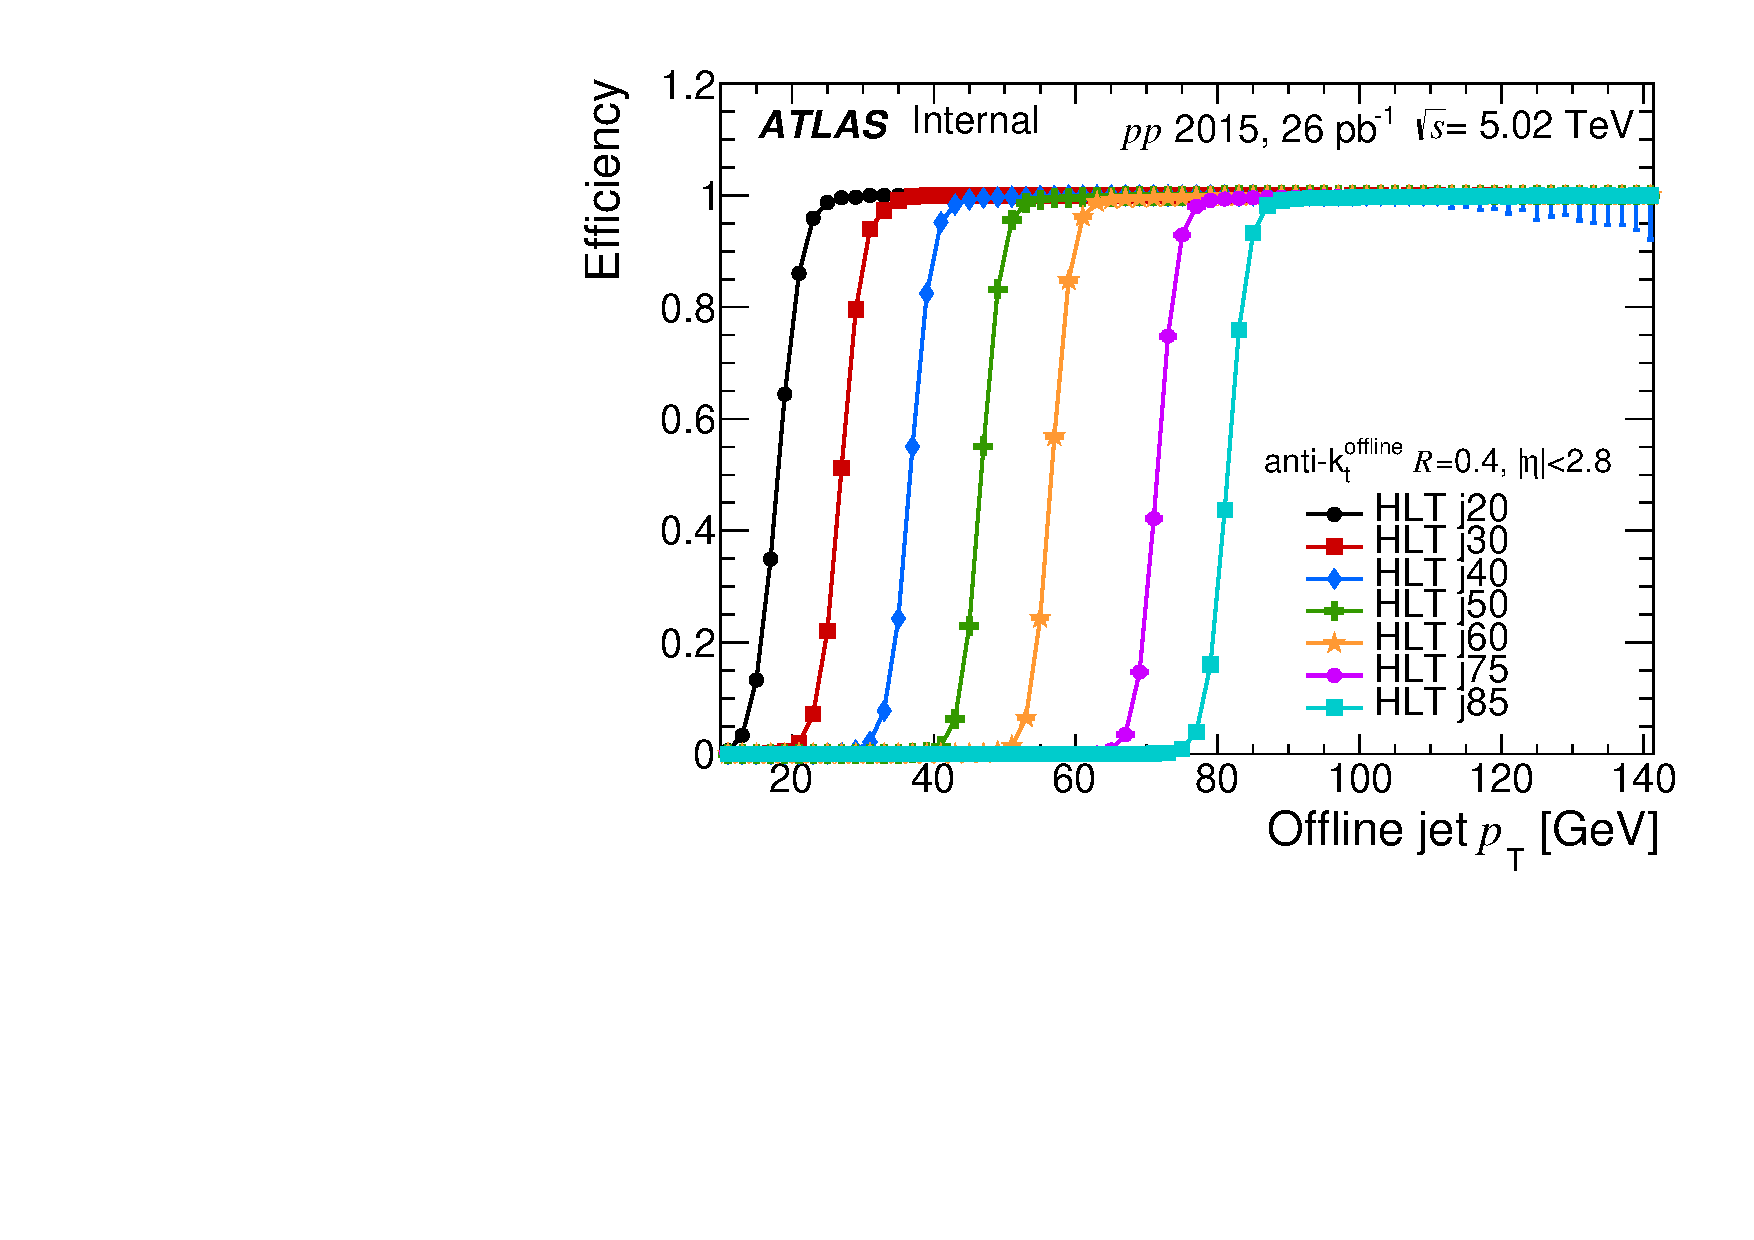
\includegraphics[width=0.45\textwidth]{figures/main/general/Eff_pp_5TeV_central.pdf} &
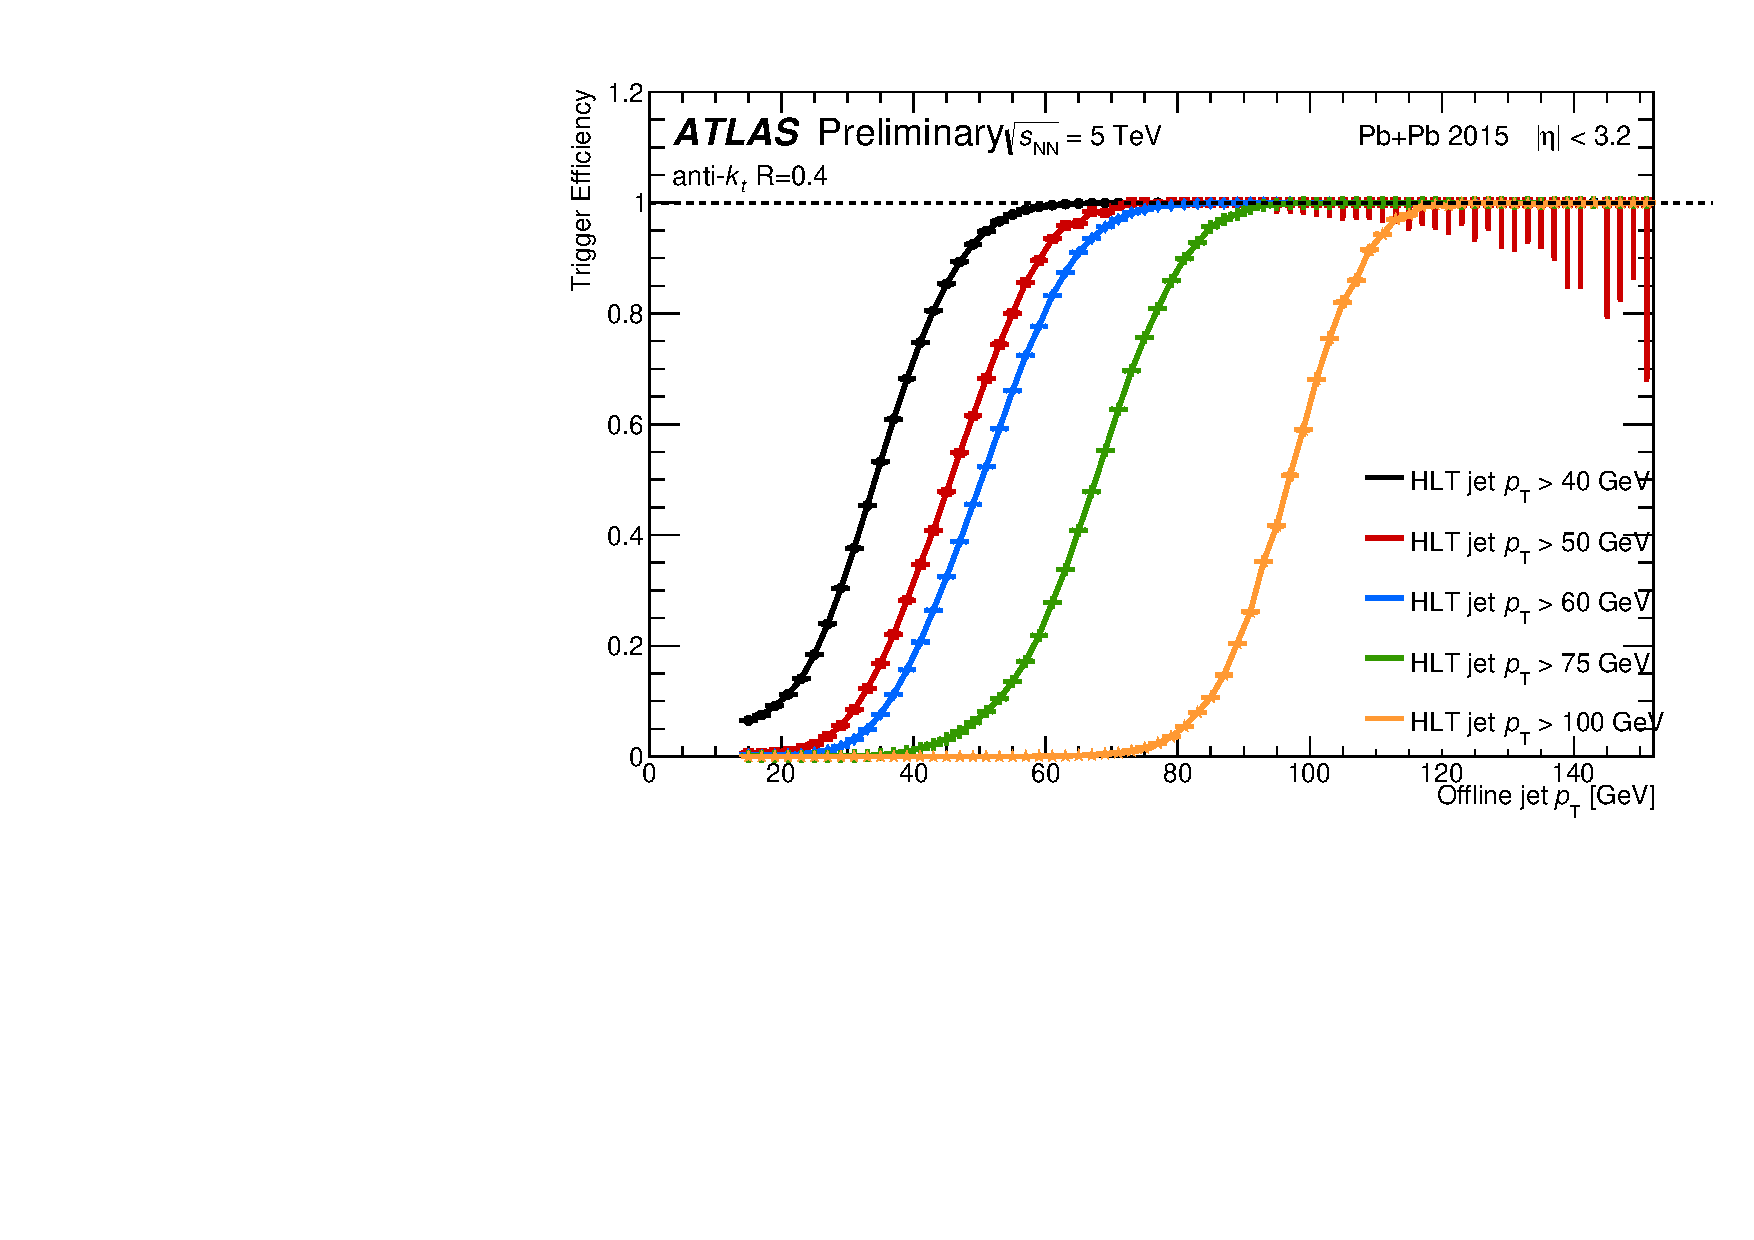
\includegraphics[width=0.45\textwidth]{figures/main/general/trigger_eff_PbPb_CentInclusive.pdf}
\end{tabular}}
\caption{Jet trigger efficiencies for (left) \pp\ and (right) 0--80\% central \pbpb\ collisions at 5.02 TeV for R=0.4 offline jets.
The broader turn-on of the jet trigger in \pbpb\ compared to \pp\ collisions is caused by significant differences between the HI jet trigger reconstruction algorithm used at the time of the data taking and the current version of the offline reconstruction software.
Figure from Ref.~\cite{Sickles:2235420} }
\label{fig:trigger_selections}
\end{figure}


%\begin{figure}
%\begin{subfigure}{.5\textwidth}
%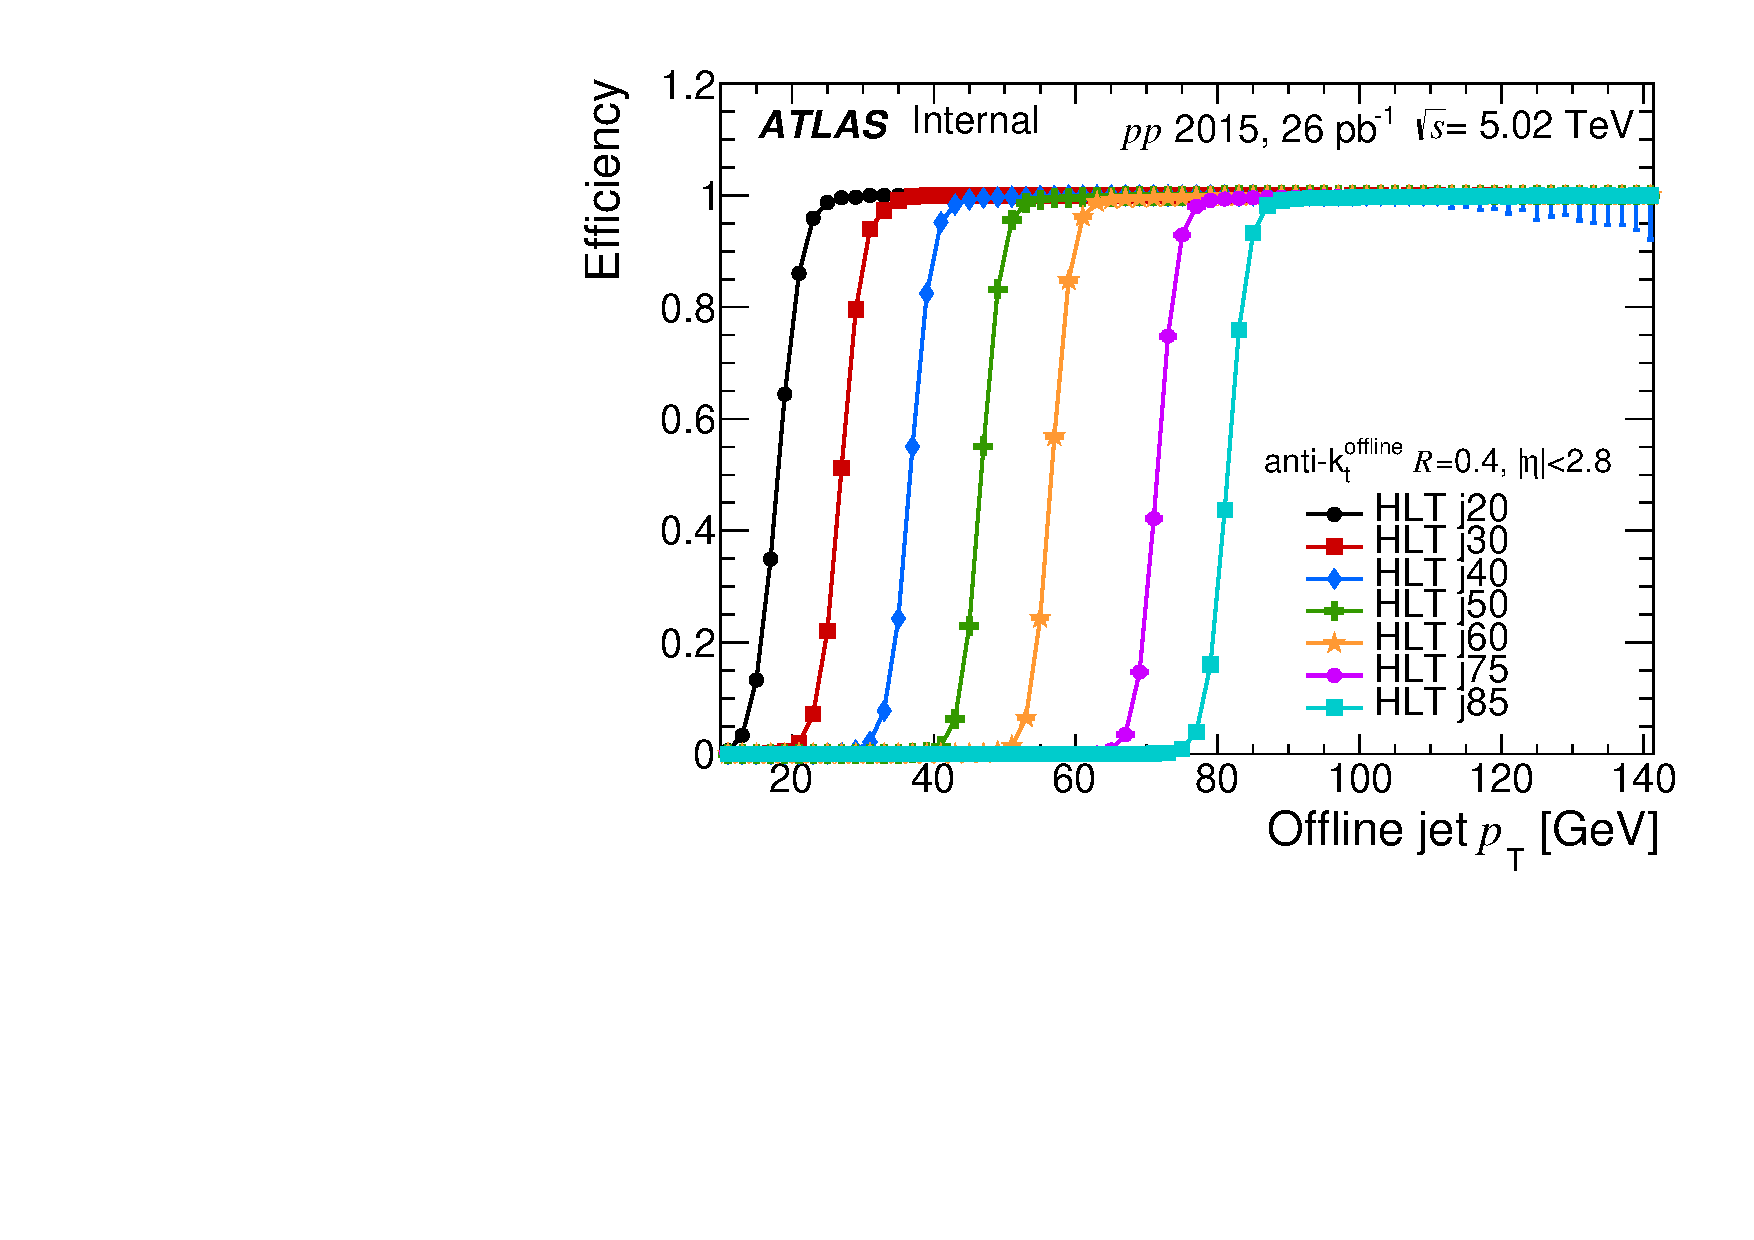
\includegraphics[width=1\textwidth]{figures/main/general/Eff_pp_5TeV_central.pdf}
%\caption{.}
%\label{fig:Trigger_pp5}
%\end{subfigure}
%\begin{subfigure}{.5\textwidth}
%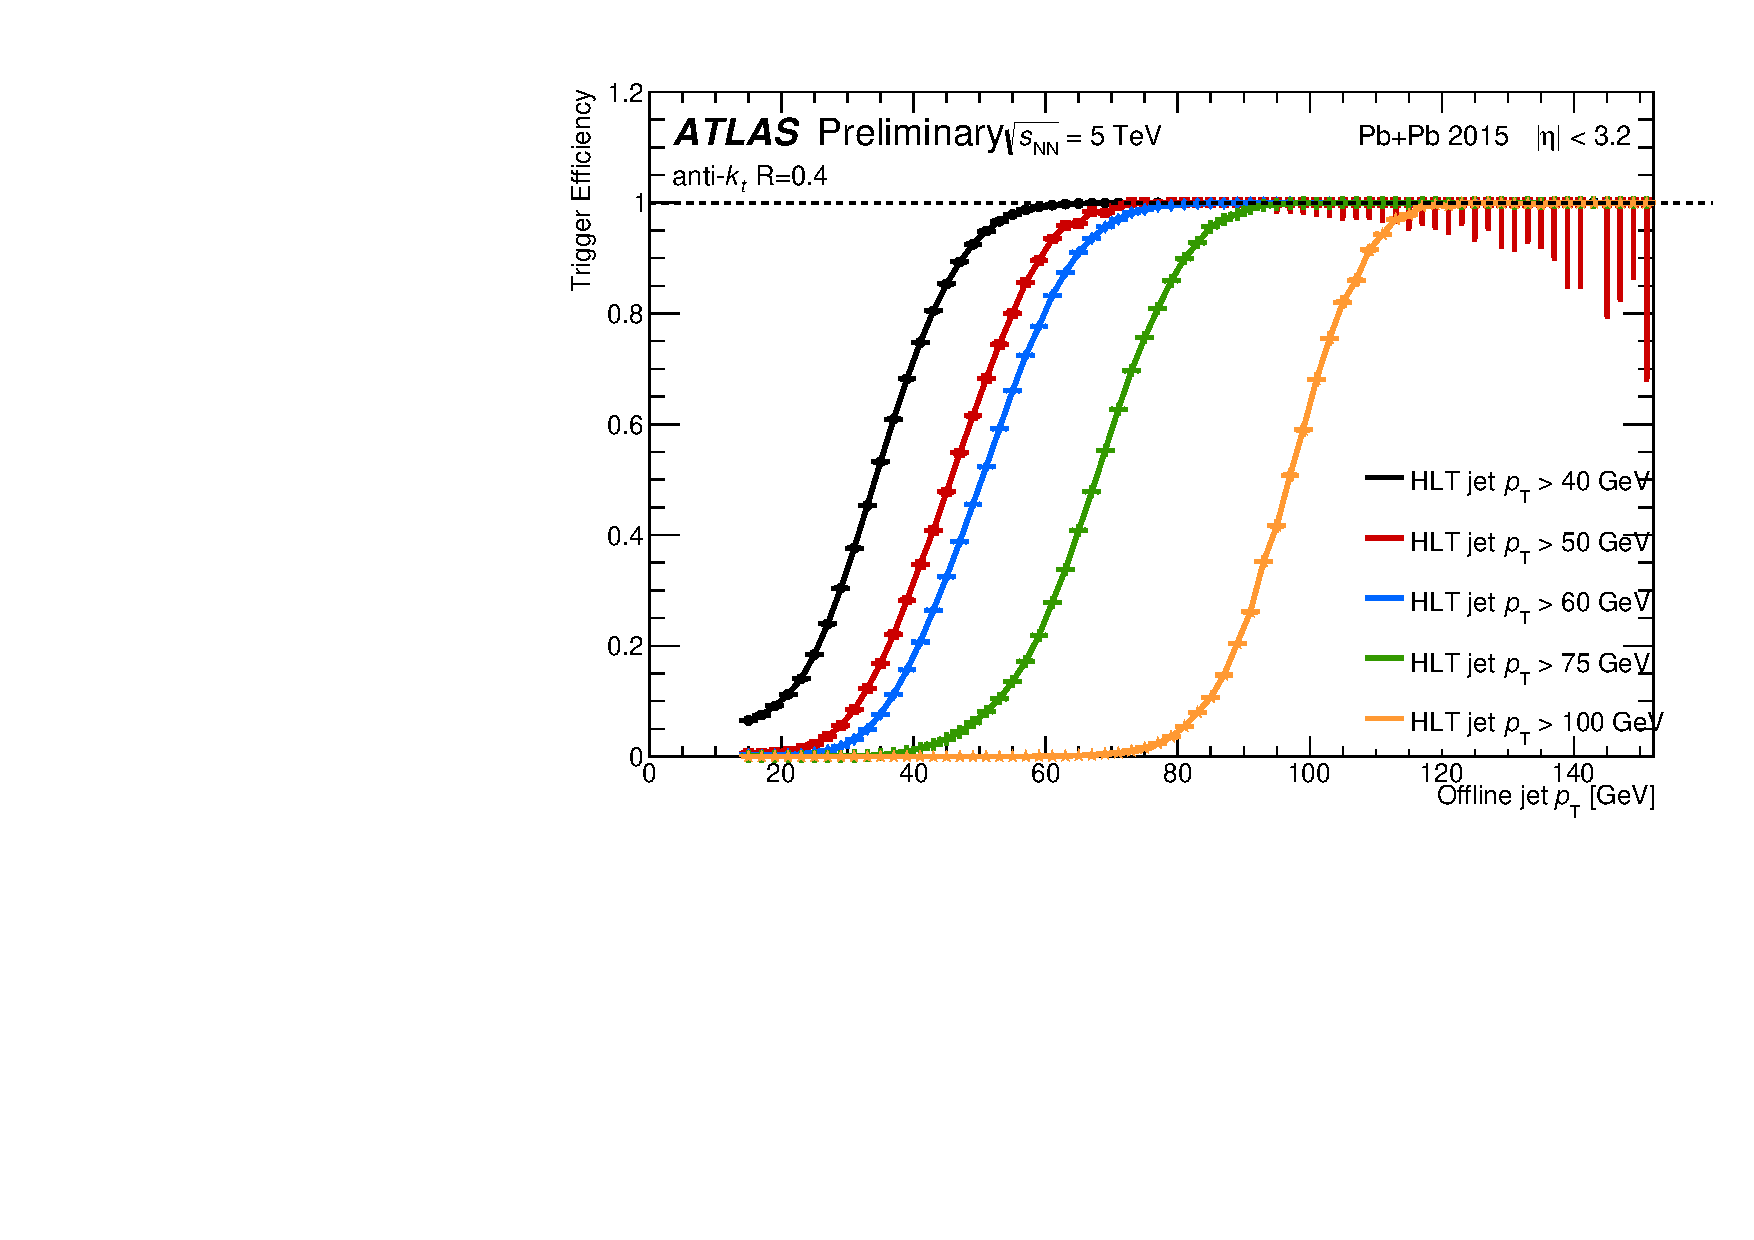
\includegraphics[width=1\textwidth]{figures/main/general/trigger_eff_PbPb_CentInclusive.pdf}
%\caption{}
%\label{fig:Trigger_PbPb}
%\end{subfigure}
%\label{fig:trigger_selections}
%\caption{Jet trigger efficiencies for (left) \pp\ and (right) 0--80\% central \pbpb\ collisions at 5.02 TeV for R=0.4 offline jets.
%The broader turn-on of the jet trigger in \pbpb\ compared to \pp\ collisions is caused by significant differences between the HI jet trigger reconstruction algorithm used at the time of the data taking and the current version of the offline reconstruction software.
%Figure from Ref.~\cite{Sickles:2235420} }
%\end{figure}

In both samples, events were required to have a reconstructed vertex within 150~mm of the nominal IP along the beam axis.
The pileup was negligible in the \pbpb\ while the \pp\ data was collected in low pileup mode, where the average number of interactions per bunch crossing in \pp\ collisions ranged from 0.6 to 1.3.
Only events taken during stable beam conditions and satisfying detector and data-quality requirements that include the detector subsystems being in nominal operating conditions were considered.
The total number of \pp\ and \pbpb\ events entering the analysis, along with the with rejection power of various event quality cuts is shown in Figure~\ref{Fig:EventCounts}.
Some of these events are rejected by multiple cuts. ``Rejection by centrality'' indicates the number of events outside the 0-80\% centrality bin.

\begin{figure}
\centerline{
\begin{tabular}{cc}
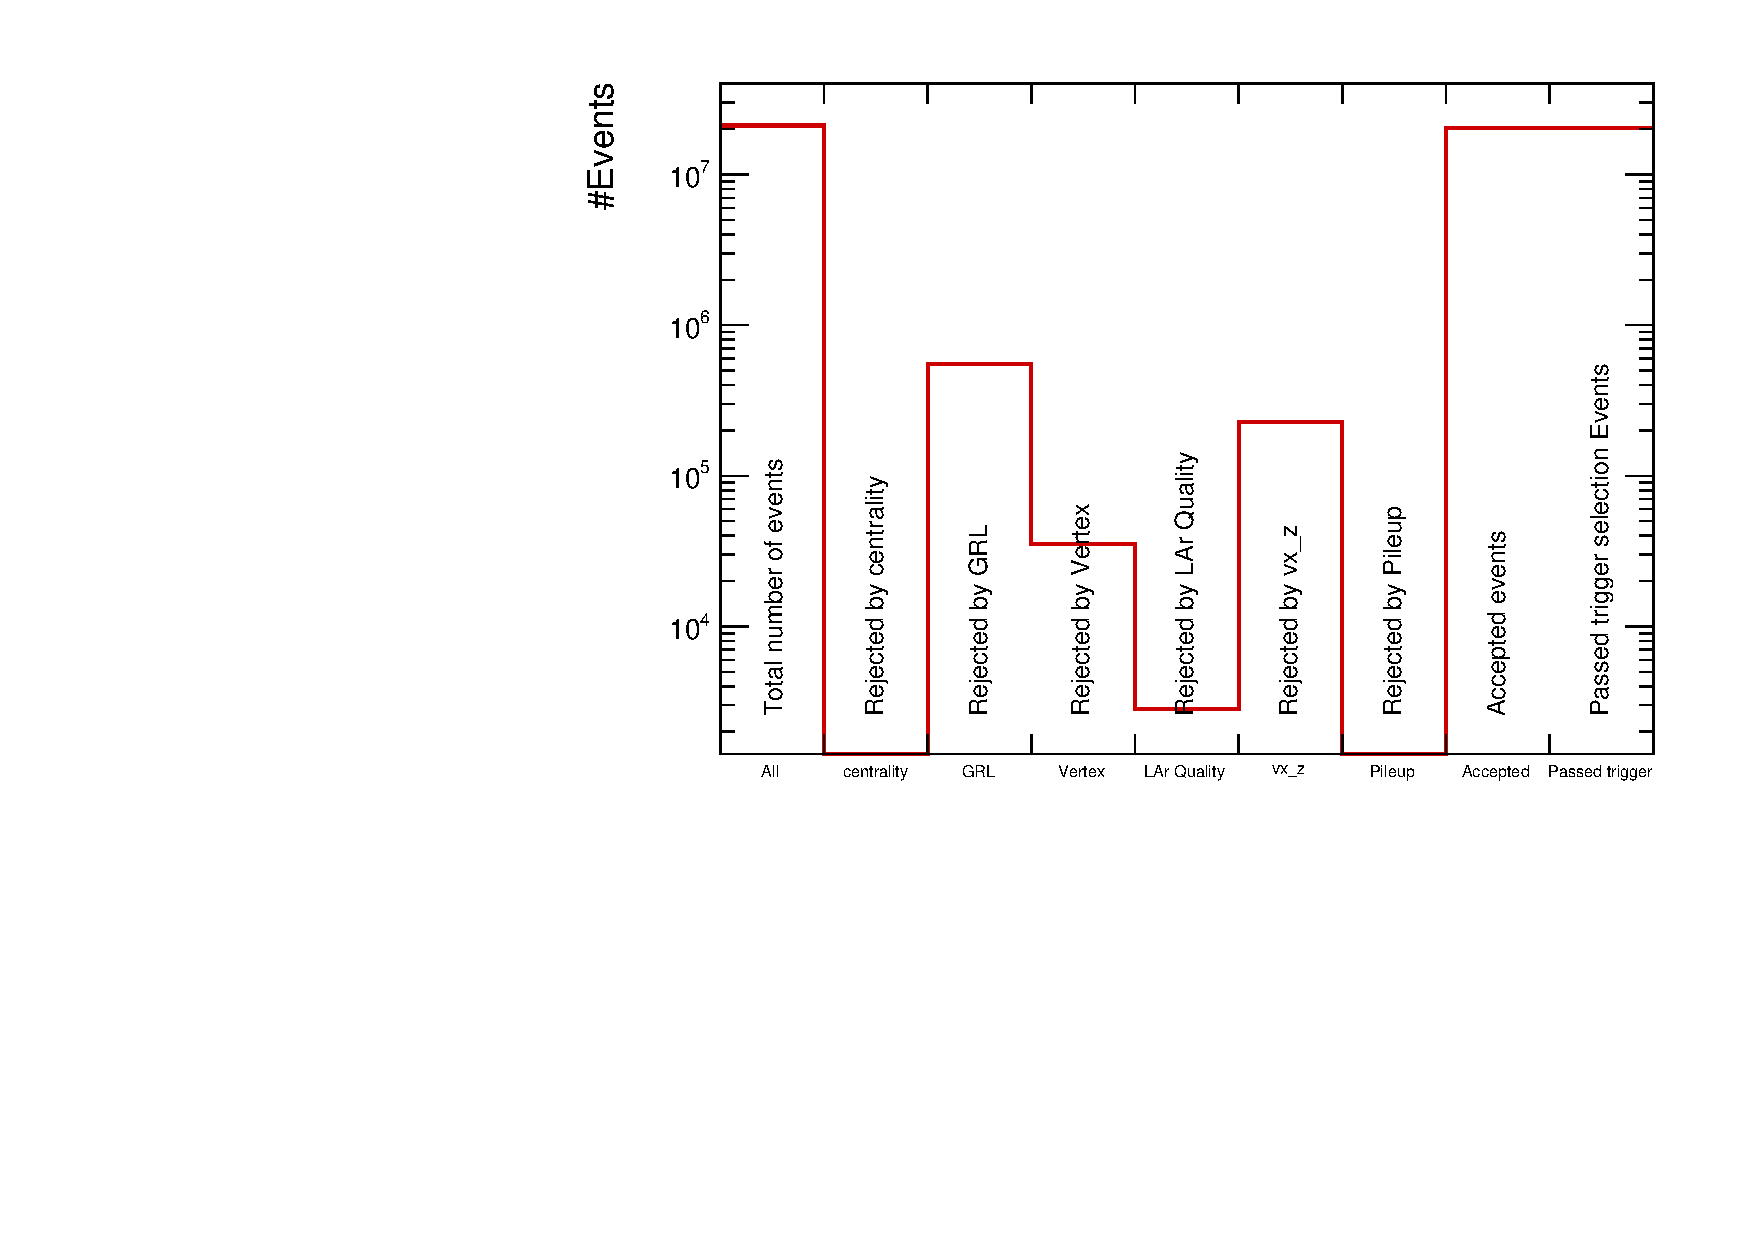
\includegraphics[width=0.45\textwidth]{figures/main/general/EventAccept_pp.pdf} & 
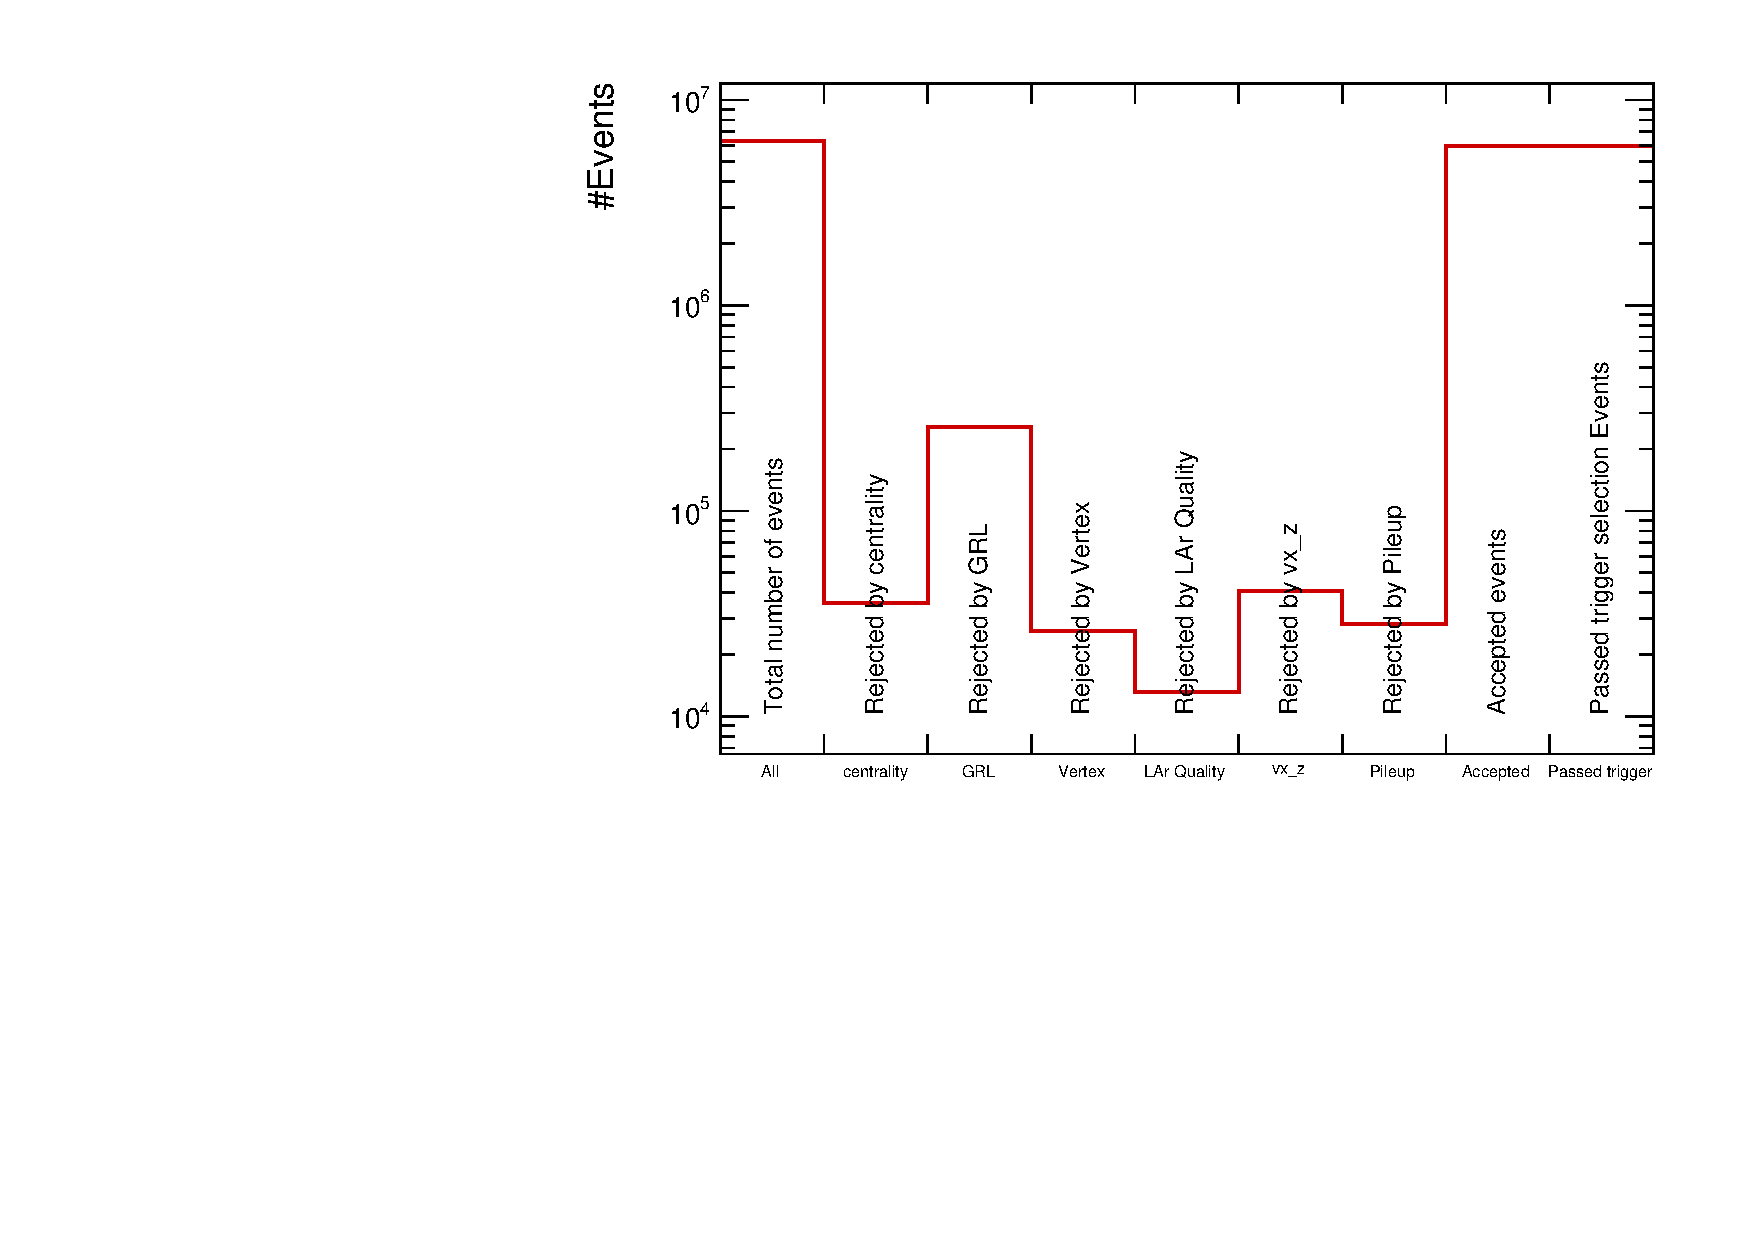
\includegraphics[width=0.45\textwidth]{figures/main/general/EventAccept_PbPb.pdf}
\end{tabular}}
\caption{The number of 2015 \pp\  (left) and \PbPb\ (right) events used and rejected by various event quality cuts.}
\label{Fig:EventCounts}
\end{figure}



The centrality intervals used in this analysis were defined according to successive percentiles of the \ETfcal\ distribution obtained in minimum bias (MB) collisions, ordered from the most central (highest \ETfcal) to the most peripheral (lowest \ETfcal) collisions: 0--10\%, 10--20\%, 20--30\%, 30--40\%, 40--60\%, 60--80\%.

The \pp\ Monte Carlo (MC) used a set of $1.8\times10^7$ 5.02 TeV hard-scattering dijet \pp\ events generated with \powheg{}+\pythiaeight\ \cite{Nason:2004rx,Sjostrand:2014zea} using the A14 tune of parameters \cite{ATLAS2014021} and the NNPDF23LO PDF set \cite{Ball:2012cx}.
The \pbpb\ MC was generated by overlaying the additional sample of MB \pbpb\ data events on a separate set of $1.8\times10^7$ 5.02 TeV hard-scattering dijet \pp\ events generated with the same tune and PDFs as the \pp\ MC.
This ``MC overlay'' sample was reweighted on an event-by-event basis such that it had the same centrality distribution as the jet triggered sample.
Another sample of MB \pbpb\ events was generated using HIJING (version 1.38b) \cite{Wang:1991hta} and was only used to evaluate the track reconstruction performance.
The detector response in all MC samples was simulated using \textsc{Geant4} \cite{Agostinelli:2002hh,Aad:2010ah}.
These MC samples were used to evaluate the performance of the detector and analysis procedure and correct the measured distributions for detector effects.


%The event fraction as a function of run number for both the hard probes stream and the minimum bias overlay stream in \pbpb\ is shown in Figure~\ref{fig:evnt_fraction}
%
%\begin{figure}[h]
%\centering
%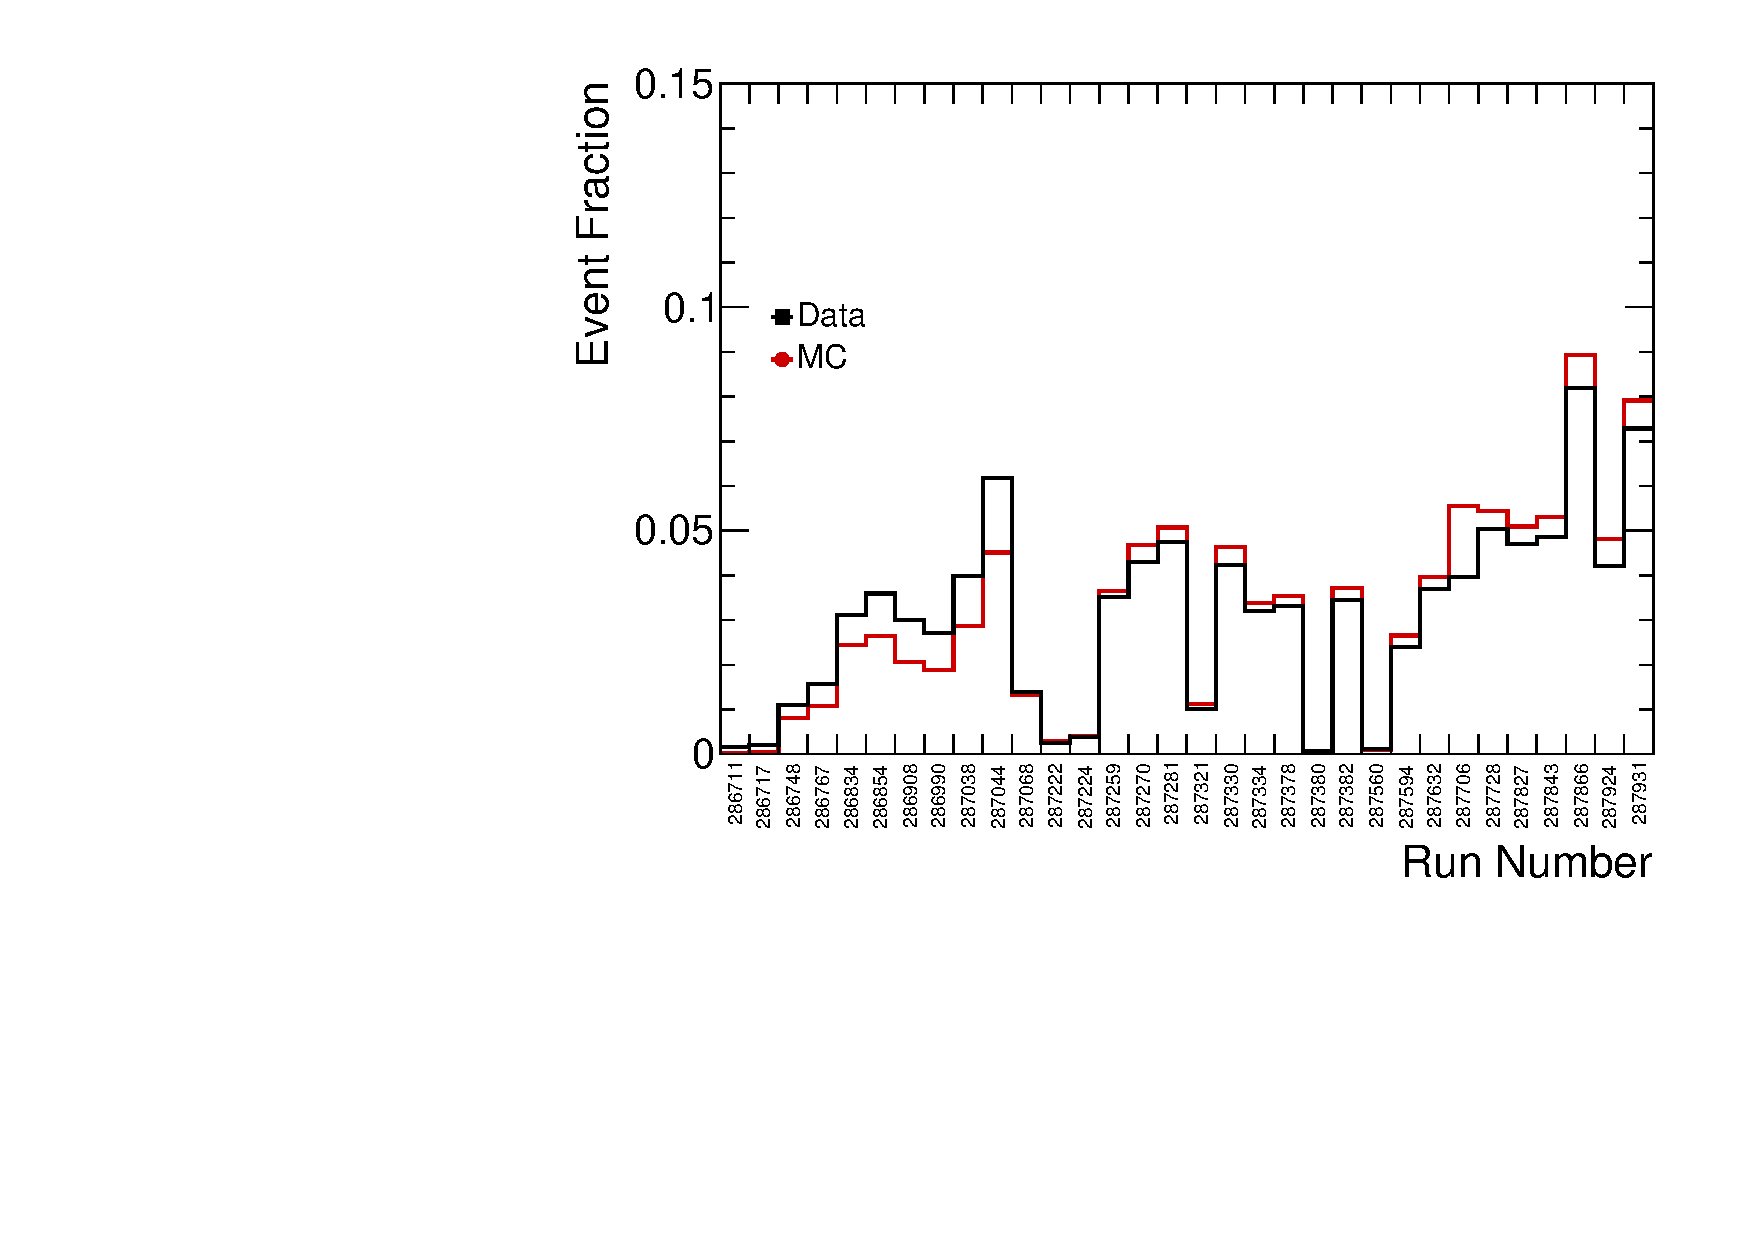
\includegraphics[width=0.5\textwidth]{figures/main/general/EventPercentages_c0.pdf}
%\caption{Event fraction as a function of runs for Hard Probes and the Minimum Bias Overlay Streams in \pbpb\ collisions.}
%\label{fig:evnt_fraction}
%\end{figure}

The time dependence of the underlying event (a core part of this measurement) was tested by dividing the data and MC into three data taking periods with approximately equal number of events in each period.
The underlying event determined for each period compared to the nominal underlying event evaluated for the entire dataset is shown in Figure~\ref{fig:weighted_runs}, and it can be seen that it is stable throughout the data taking period.

 \begin{figure}[h]
\centering
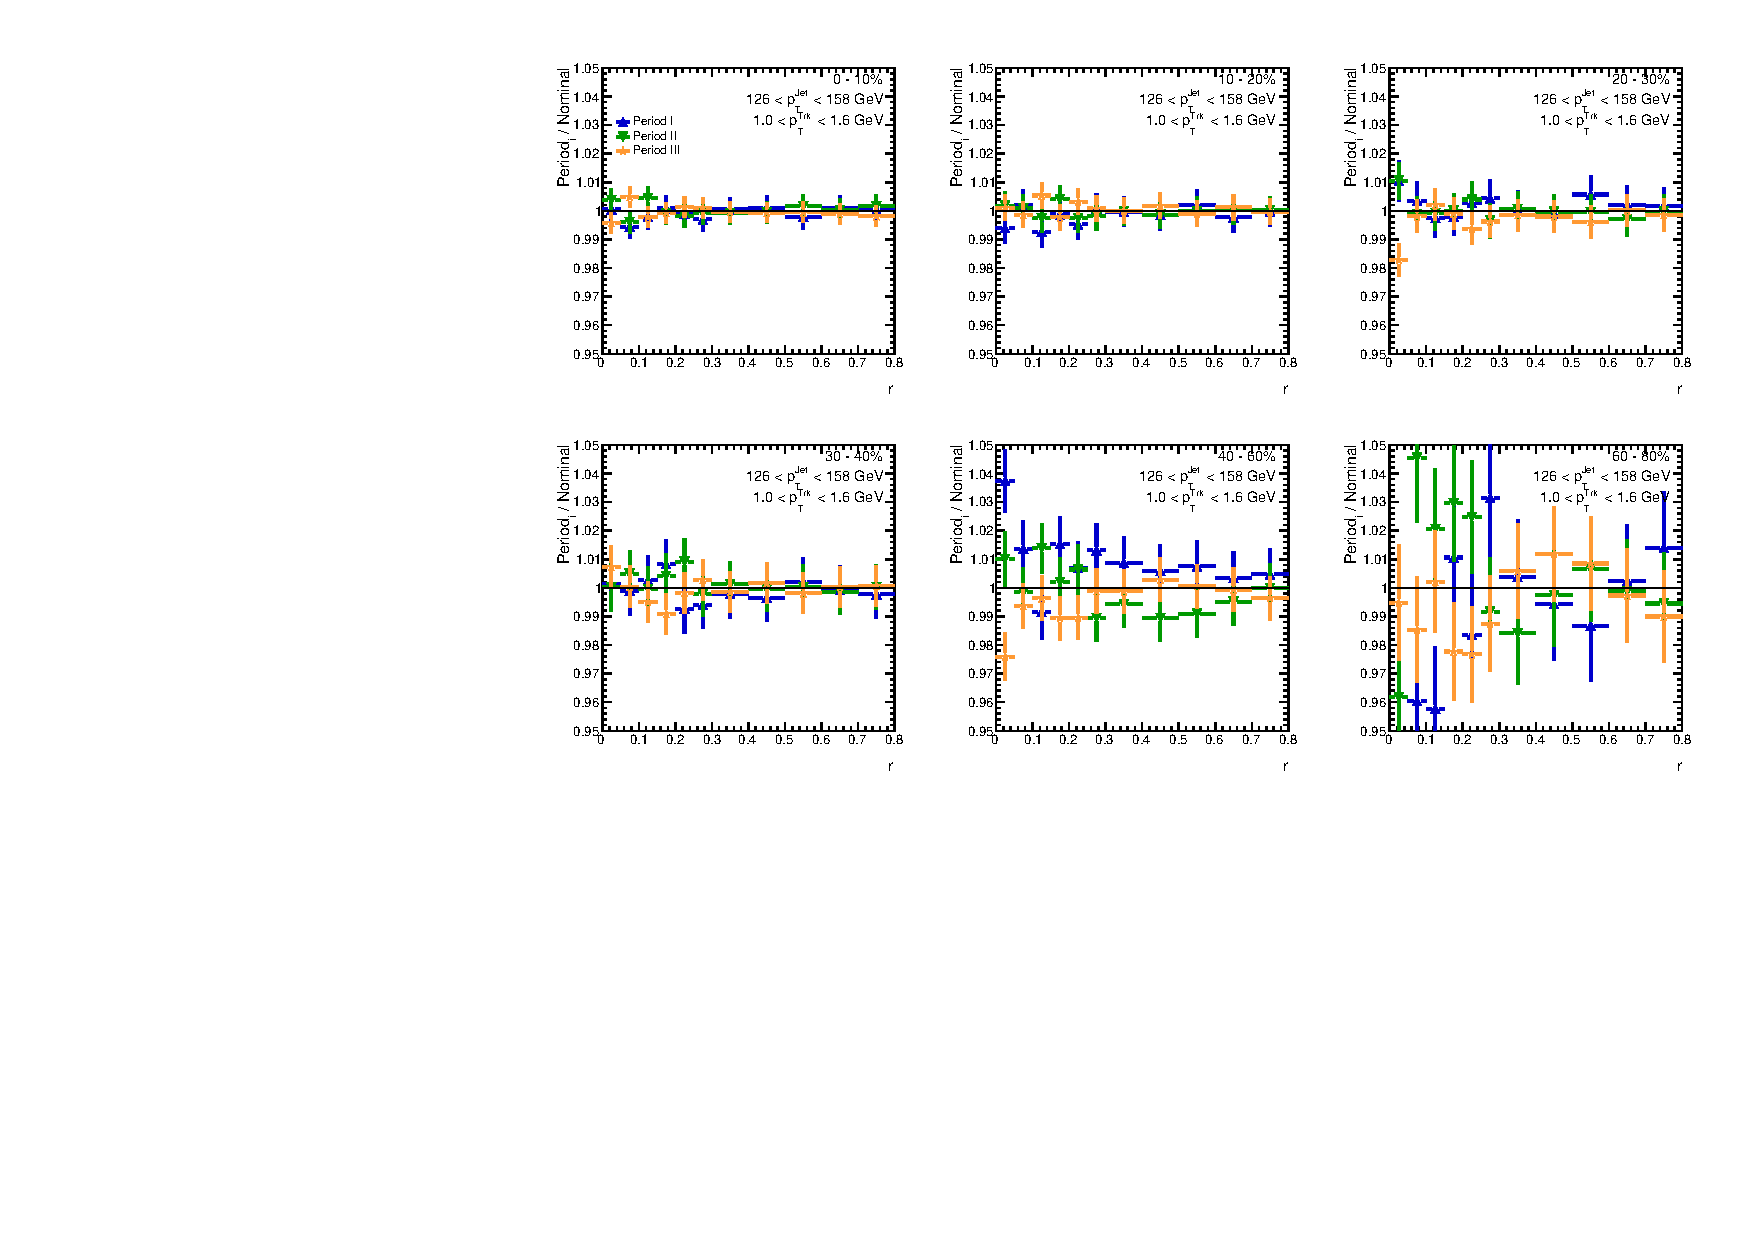
\includegraphics[width=0.75\textwidth]{figures/main/general/weightedRuns.pdf}
\caption{Stability of the underlying event for three different periods of the data taking.
The different curves indicate the ratio of the underlying event in each period of data taking to the underlying event determined in the entire dataset.}
\label{fig:weighted_runs}
\end{figure}





